% Created 2020-05-13 三 11:02
% Intended LaTeX compiler: pdflatex
\documentclass[11pt]{article}
\usepackage[utf8]{inputenc}
\usepackage[T1]{fontenc}
\usepackage{graphicx}
\usepackage{grffile}
\usepackage{longtable}
\usepackage{wrapfig}
\usepackage{rotating}
\usepackage[normalem]{ulem}
\usepackage{amsmath}
\usepackage{textcomp}
\usepackage{amssymb}
\usepackage{capt-of}
\usepackage{imakeidx}
\usepackage{hyperref}
\usepackage{minted}
% TIPS
% \substack{a\\b} for multiple lines text





% pdfplots will load xolor automatically without option
\usepackage[dvipsnames]{xcolor}

\usepackage{forest}
% two-line text in node by [two \\ lines]
% \begin{forest} qtree, [..] \end{forest}
\forestset{
  qtree/.style={
    baseline,
    for tree={
      parent anchor=south,
      child anchor=north,
      align=center,
      inner sep=1pt,
    }}}
%\usepackage{flexisym}
% load order of mathtools and mathabx, otherwise conflict overbrace

\usepackage{mathtools}
%\usepackage{fourier}
\usepackage{pgfplots}
\usepackage{amsthm}
\usepackage{amsmath}
%\usepackage{unicode-math}
%
\usepackage{commath}
%\usepackage{,  , }
\usepackage{amsfonts}
\usepackage{amssymb}
% importing symbols https://tex.stackexchange.com/questions/14386/importing-a-single-symbol-from-a-different-font
%mathabx change every symbol
% use instead stmaryrd
%\usepackage{mathabx}
\usepackage{stmaryrd}
\usepackage{empheq}
\usepackage{tikz}
\usepackage{tikz-cd}
%\usepackage[notextcomp]{stix}
\usetikzlibrary{arrows.meta}
\usepackage[most]{tcolorbox}
%\utilde
%\usepackage{../../latexpackage/undertilde/undertilde}
% left and right superscript and subscript
\usepackage{actuarialsymbol}
\usepackage{threeparttable}
\usepackage{scalerel,stackengine}
\usepackage{stackrel}
% \stackrel[a]{b}{c}
\usepackage{dsfont}
% text font
\usepackage{newpxtext}
%\usepackage{newpxmath}

%\newcounter{dummy} \numberwithin{dummy}{section}
\newtheorem{dummy}{dummy}[section]
\theoremstyle{definition}
\newtheorem{definition}[dummy]{Definition}
\newtheorem{corollary}[dummy]{Corollary}
\newtheorem{lemma}[dummy]{Lemma}
\newtheorem{proposition}[dummy]{Proposition}
\newtheorem{theorem}[dummy]{Theorem}
\theoremstyle{definition}
\newtheorem{example}[dummy]{Example}
\theoremstyle{remark}
\newtheorem*{remark}{Remark}


\newcommand\what[1]{\ThisStyle{%
    \setbox0=\hbox{$\SavedStyle#1$}%
    \stackengine{-1.0\ht0+.5pt}{$\SavedStyle#1$}{%
      \stretchto{\scaleto{\SavedStyle\mkern.15mu\char'136}{2.6\wd0}}{1.4\ht0}%
    }{O}{c}{F}{T}{S}%
  }
}

\newcommand\wtilde[1]{\ThisStyle{%
    \setbox0=\hbox{$\SavedStyle#1$}%
    \stackengine{-.1\LMpt}{$\SavedStyle#1$}{%
      \stretchto{\scaleto{\SavedStyle\mkern.2mu\AC}{.5150\wd0}}{.6\ht0}%
    }{O}{c}{F}{T}{S}%
  }
}

\newcommand\wbar[1]{\ThisStyle{%
    \setbox0=\hbox{$\SavedStyle#1$}%
    \stackengine{.5pt+\LMpt}{$\SavedStyle#1$}{%
      \rule{\wd0}{\dimexpr.3\LMpt+.3pt}%
    }{O}{c}{F}{T}{S}%
  }
}

\newcommand{\bl}[1] {\boldsymbol{#1}}
\newcommand{\Wt}[1] {\stackrel{\sim}{\smash{#1}\rule{0pt}{1.1ex}}}
\newcommand{\wt}[1] {\widetilde{#1}}
\newcommand{\tf}[1] {\textbf{#1}}


%For boxed texts in align, use Aboxed{}
%otherwise use boxed{}

\DeclareMathSymbol{\widehatsym}{\mathord}{largesymbols}{"62}
\newcommand\lowerwidehatsym{%
  \text{\smash{\raisebox{-1.3ex}{%
    $\widehatsym$}}}}
\newcommand\fixwidehat[1]{%
  \mathchoice
    {\accentset{\displaystyle\lowerwidehatsym}{#1}}
    {\accentset{\textstyle\lowerwidehatsym}{#1}}
    {\accentset{\scriptstyle\lowerwidehatsym}{#1}}
    {\accentset{\scriptscriptstyle\lowerwidehatsym}{#1}}
}

\usepackage{graphicx}
    
% text on arrow for xRightarrow
\makeatletter
%\newcommand{\xRightarrow}[2][]{\ext@arrow 0359\Rightarrowfill@{#1}{#2}}
\makeatother


\newcommand{\dom}[1]{%
\mathrm{dom}{(#1)}
}

% Roman numerals
\makeatletter
\newcommand*{\rom}[1]{\expandafter\@slowromancap\romannumeral #1@}
\makeatother

\def \fR {\mathfrak{R}}
\def \bx {\boldsymbol{x}}
\def \bz {\boldsymbol{z}}
\def \ba {\boldsymbol{a}}
\def \bh {\boldsymbol{h}}
\def \bo {\boldsymbol{o}}
\def \bU {\boldsymbol{U}}
\def \bc {\boldsymbol{c}}
\def \bV {\boldsymbol{V}}
\def \bI {\boldsymbol{I}}
\def \bK {\boldsymbol{K}}
\def \bt {\boldsymbol{t}}
\def \bb {\boldsymbol{b}}
\def \bA {\boldsymbol{A}}
\def \bX {\boldsymbol{X}}
\def \bu {\boldsymbol{u}}
\def \bS {\boldsymbol{S}}
\def \bZ {\boldsymbol{Z}}
\def \bz {\boldsymbol{z}}
\def \by {\boldsymbol{y}}
\def \bw {\boldsymbol{w}}
\def \bT {\boldsymbol{T}}
\def \bF {\boldsymbol{F}}
\def \bS {\boldsymbol{S}}
\def \bm {\boldsymbol{m}}
\def \bW {\boldsymbol{W}}
\def \bR {\boldsymbol{R}}
\def \bQ {\boldsymbol{Q}}
\def \bS {\boldsymbol{S}}
\def \bP {\boldsymbol{P}}
\def \bT {\boldsymbol{T}}
\def \bY {\boldsymbol{Y}}
\def \bH {\boldsymbol{H}}
\def \bB {\boldsymbol{B}}
\def \blambda {\boldsymbol{\lambda}}
\def \bPhi {\boldsymbol{\Phi}}
\def \btheta {\boldsymbol{\theta}}
\def \bTheta {\boldsymbol{\Theta}}
\def \bmu {\boldsymbol{\mu}}
\def \bphi {\boldsymbol{\phi}}
\def \bSigma {\boldsymbol{\Sigma}}
\def \lb {\left\{}
\def \rb {\right\}}
\def \la {\langle}
\def \ra {\rangle}
\def \caln {\mathcal{N}}
\def \dissum {\displaystyle\Sigma}
\def \dispro {\displaystyle\prod}
\def \E {\mathbb{E}}
\def \Q {\mathbb{Q}}
\def \N {\mathbb{N}}
\def \V {\mathbb{V}}
\def \R {\mathbb{R}}
\def \P {\mathbb{P}}
\def \A {\mathbb{A}}
\def \Z {\mathbb{Z}}
\def \I {\mathbb{I}}
\def \C {\mathbb{C}}
\def \cala {\mathcal{A}}
\def \calb {\mathcal{B}}
\def \calq {\mathcal{Q}}
\def \calp {\mathcal{P}}
\def \cals {\mathcal{S}}
\def \calg {\mathcal{G}}
\def \caln {\mathcal{N}}
\def \calr {\mathcal{R}}
\def \calm {\mathcal{M}}
\def \calc {\mathcal{C}}
\def \calf {\mathcal{F}}
\def \calk {\mathcal{K}}
\def \call {\mathcal{L}}
\def \calu {\mathcal{U}}
\def \bcup {\bigcup}


\def \uin {\underline{\in}}
\def \oin {\overline{\in}}
\def \uR {\underline{R}}
\def \oR {\overline{R}}
\def \uP {\underline{P}}
\def \oP {\overline{P}}

\def \Ra {\Rightarrow}

\def \e {\enspace}

\def \sgn {\operatorname{sgn}}
\def \gen {\operatorname{gen}}
\def \ker {\operatorname{ker}}
\def \im {\operatorname{im}}

\def \tril {\triangleleft}

% \varprod
\DeclareSymbolFont{largesymbolsA}{U}{txexa}{m}{n}
\DeclareMathSymbol{\varprod}{\mathop}{largesymbolsA}{16}

% \bigtimes
\DeclareFontFamily{U}{mathx}{\hyphenchar\font45}
\DeclareFontShape{U}{mathx}{m}{n}{
      <5> <6> <7> <8> <9> <10>
      <10.95> <12> <14.4> <17.28> <20.74> <24.88>
      mathx10
      }{}
\DeclareSymbolFont{mathx}{U}{mathx}{m}{n}
\DeclareMathSymbol{\bigtimes}{1}{mathx}{"91}
% \odiv
\DeclareFontFamily{U}{matha}{\hyphenchar\font45}
\DeclareFontShape{U}{matha}{m}{n}{
      <5> <6> <7> <8> <9> <10> gen * matha
      <10.95> matha10 <12> <14.4> <17.28> <20.74> <24.88> matha12
      }{}
\DeclareSymbolFont{matha}{U}{matha}{m}{n}
\DeclareMathSymbol{\odiv}         {2}{matha}{"63}


\newcommand\subsetsim{\mathrel{%
  \ooalign{\raise0.2ex\hbox{\scalebox{0.9}{$\subset$}}\cr\hidewidth\raise-0.85ex\hbox{\scalebox{0.9}{$\sim$}}\hidewidth\cr}}}
\newcommand\simsubset{\mathrel{%
  \ooalign{\raise-0.2ex\hbox{\scalebox{0.9}{$\subset$}}\cr\hidewidth\raise0.75ex\hbox{\scalebox{0.9}{$\sim$}}\hidewidth\cr}}}

\newcommand\simsubsetsim{\mathrel{%
  \ooalign{\raise0ex\hbox{\scalebox{0.8}{$\subset$}}\cr\hidewidth\raise1ex\hbox{\scalebox{0.75}{$\sim$}}\hidewidth\cr\raise-0.95ex\hbox{\scalebox{0.8}{$\sim$}}\cr\hidewidth}}}
\newcommand{\stcomp}[1]{{#1}^{\mathsf{c}}}


\author{Stanley Burris \& H. P. Sankappanavar}
\date{\today}
\title{A Course In Universal Algebra}
\hypersetup{
 pdfauthor={Stanley Burris \& H. P. Sankappanavar},
 pdftitle={A Course In Universal Algebra},
 pdfkeywords={},
 pdfsubject={},
 pdfcreator={Emacs 26.3 (Org mode 9.3.6)}, 
 pdflang={English}}
\begin{document}

\maketitle \clearpage
\tableofcontents \clearpage
\section{Lattices}
\label{sec:org9b69538}

\subsection{Definitions of Lattices}
\label{sec:org713f090}
\begin{definition}[]
A nonempty set \(L\) together with two binary operations \(\vee\) and \(\wedge\)
(read "join" and "meet" respectively) on \(L\) is called a \textbf{lattice} if it
satisfies the following identities
\begin{itemize}%[leftmargin=6em]
 \item[L1:] (a) $x\vee y\approx y\vee x$ \par
 (b) $x\wedge y\approx y\wedge x$\hspace*{\fill}(commutative laws)
 \item[L2:] (a) $x\vee(y\vee z)\approx(x\vee y)\vee z$ \par 
 (b) $x\wedge(y\wedge z)\approx(x\wedge y)\wedge z$
 \hspace*{\fill}(associate laws)
 \item[L3:] (a) \(x\vee x\approx x\)\par 
 (b) \(x\wedge x\approx x\)
 \hspace*{\fill}(idempotent laws)
 \item[L4:] (a) \(x\approx x\vee(x\wedge y)\)\par 
 (b) \(x\approx x\wedge(x\vee y)\)
 \hspace*{\fill}(absorption laws)
\end{itemize}
\end{definition}

\begin{definition}[]
Let \(A\) be a subset of a poset \(P\). An element \(p\) in \(P\) is an \textbf{upper bound}
for \(A\) if \(a\le p\) for every \(a\) in \(A\). An element \(p\) in \(P\) is the
\textbf{least upper bound} of \(A\) (l.u.b. of \(A\)) or \textbf{supremum} of \(A\) (\(\sup A\).

For \(a,b\) in \(P\) we say \(b\) \textbf{covers} \(a\), or \(a\) is \textbf{covered by} \(b\) if
\(a<b\) and whenever \(a\le c\le b\) it follows that \(a=c\) or \(c=b\). We
use the notation \(a\prec b\) to denote \(a\) is covered by \(b\). 
\end{definition}

\begin{definition}[]
A poset \(L\) is a lattice iff for every \(a,b\) in \(L\) both \(\sup\{a,b\}\)
and \(\inf\{a,b\}\) exist
\end{definition}

\begin{enumerate}
\item If \(L\) is a lattice by the first definition, then define \(\le\) on \(L\)
by \(a\le b\) iff \(a=a\wedge b\)
\item If \(L\) is a lattice by the second definition, then define \(\vee\) and
\(\wedge\) by \(a\vee b=\sup\{a,b\}\) and \(a\wedge b=\inf\{a,b\}\)
\end{enumerate}


\subsection{Isomorphism Lattices, and Sublattices}
\label{sec:orgaf64f00}
\begin{definition}[]
Two lattices \(L_1\) and \(L_2\) are \textbf{isomorphic} if there is a bijection
\(\alpha\) from \(L_1\) to \(L_2\) s.t. for every \(a,b\) in \(L_1\) the following two
equation hold: \(\alpha(a\vee b)=\alpha(a)\vee\alpha(b)\) and 
\(\alpha(a\wedge b)=\alpha(a)\wedge\alpha(b)\). Such an \(\alpha\) is called an \textbf{isomorphism}
\end{definition}

\begin{definition}[]
If \(P_1\) and \(P_2\) are two posets and \(\alpha\) is a map from \(P_1\) to \(P_2\), then we
say \(\alpha\) is \textbf{order-preserving} if \(\alpha(a)\le\alpha(b)\) holds in \(P_2\) whenever
\(a\le b\) holds in \(P_1\)
\end{definition}

\begin{theorem}[]
Two lattices \(L_1\) and \(L_2\) are isomorphic iff there is a bijection \(\alpha\) from
\(L_1\) to \(L_2\) s.t. both \(\alpha\) and \(\alpha^{-1}\) are order-preserving
\end{theorem}

\begin{definition}[]
If \(L\) is a lattice and \(L'\neq\emptyset\) is a subset of \(L\) s.t. for every
pair of elements \(a,b\) in \(L'\) both \(a\vee b\) and \(a\wedge b\) are in
\(L'\), where \(\wedge,\vee\) are the lattice operations of \(L\), then we say
that \(L'\) with the same operations is a \textbf{sublattice} of \(L\)
\end{definition}

\begin{definition}[]
A lattice \(L_1\) can be \textbf{embedded} into a lattice \(L_2\) if there is a sublattice
of \(L_2\) isomorphic to \(L_1\); in this case we also say that \(L_2\) 
\textbf{contains a copy of \(L_1\) as a sublattice}
\end{definition}

\subsection{Distributive and Modular Lattices}
\label{sec:org6c36a0e}
\begin{definition}[]
A \textbf{distributive lattice} is a lattice which satisfies either  of the
distributive laws,
\begin{itemize}
\item[D1:] \(x\wedge(y\vee z)\approx(x\wedge y)\vee(x\wedge z)\)
\item[D2:] \(x\vee(y\wedge z)\approx(x\vee y)\wedge(x\vee z)\)
\end{itemize}
\end{definition}

\begin{theorem}[]
A lattice \(L\) satisfies D1 iff it satisfies D2
\begin{align*}
x\vee(y\wedge z)&\approx(x\vee(x\wedge z))\vee(y\wedge z)\tag*{(by L4(a))}\\
&\approx x\vee((x\wedge z)\vee(y\wedge z))\\
&\approx x\vee((z\wedge x)\vee(z\wedge y))\\
&\approx x\vee(z\wedge(x\vee y))\\
&\approx x\vee((x\vee y)\wedge z)\\
&\approx (x\wedge(x\vee y))\vee(x\vee y\wedge z)\\
&\approx ((x\vee y)\wedge x)\vee((x\vee y)\wedge)\\
&\approx (x\vee y)\wedge(x\vee z)
\end{align*}
\end{theorem}

Actually every lattice satisfies both of the inequalities
\((x\wedge y)\vee(x\wedge z)\le x\wedge(y\vee z)\) and
\(x\vee(y\wedge z)\le(x\vee y)\wedge(x\vee z)\).

\begin{definition}[]
A \textbf{modular lattice} is any lattice which satisfies the \textbf{modular} law
\begin{itemize}
\item[M:] \(x\le y\to x\vee(y\wedge z)\approx y\wedge(x\vee z)\)
\end{itemize}
\end{definition}
Equivalent to the identity
\begin{equation*}
(x\wedge y)\vee(y\wedge z)\approx y\wedge((x\wedge y)\vee z)
\end{equation*}
Every lattice satisfies
\begin{equation*}
x\le y\to x\vee(y\wedge z)\le y\wedge(x\vee z)
\end{equation*}

\begin{theorem}[]
Every distributive lattice is a modular lattice
\end{theorem}

Neither \(M_5\) nor \(N_5\) is a distributive lattice in Figure \ref{fig:mn}

\begin{figure}
\centering
\begin{subfigure}[b]{0.3\textwidth}
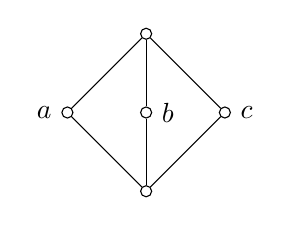
\begin{tikzpicture}
[dot/.style={circle,draw,minimum width=4pt,inner sep=1pt}]
\node[dot,label=left:$a$] (a) at (0,0) {};
\node[dot,label=right:$b$] (b) at (1,0) {};
\node[dot,label=right:$c$] (c) at (2,0) {};
\node[dot] (d) at (1,-1) {};
\node[dot] (e) at (1,1) {};
\path[] (e) edge (a) edge (b) edge (c)
(d) edge (a) edge (b) edge (c);
\end{tikzpicture}
\caption*{$M_5$}
\end{subfigure}
\begin{subfigure}[b]{0.3\textwidth}
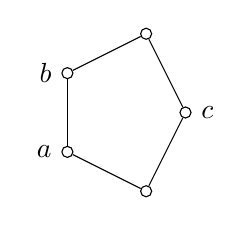
\begin{tikzpicture}
[dot/.style={circle,draw,minimum width=4pt,inner sep=1pt}]
\node[dot,label=left:$a$] (a) at (0,-0.5) {};
\node[dot,label=left:$b$] (b) at (0,0.5) {};
\node[dot,label=right:$c$] (c) at (1.5,0) {};
\node[dot] (d) at (1,1) {};
\node[dot] (e) at (1,-1) {};
\path (d) edge (b) edge (c)
(b) edge (a) 
(e) edge (a) edge (c);
\end{tikzpicture}
\caption*{$N_5$}
\end{subfigure}
\caption{}
\label{fig:mn}
\end{figure}

\begin{theorem}[Dedekind]
\label{thm3.5}
\(L\) is a nonmodular lattice iff \(N_5\) can be embedded into \(L\)
\end{theorem}

\begin{proof}
If \(L\) doesn't satisfy the modular law. Then for some \(a,b,c\) in \(L\) we
have \(a\le b\) but \(a\vee(b\wedge c)<b\wedge(a\vee c)\). Let
\(a_1=a\vee(b\wedge c)\) and \(b_1=b\wedge(a\vee c)\). Then
\begin{equation*}
c\wedge b_1=c\wedge(b\wedge(a\vee c))=(c\wedge(a\vee c))\wedge b=c\wedge b
\end{equation*}
and
\begin{equation*}
c\vee a_1=c\vee a
\end{equation*}
Now as \(c\wedge b\le a_1\le b_1\), we have \(c\wedge b\le c\wedge a_1\le
   c\wedge b_1=c\wedge b\), hence \(c\wedge a_1=c\wedge b\). Likewise
\(c\vee a=c\vee b_1\)
\begin{figure}[H]
\centering
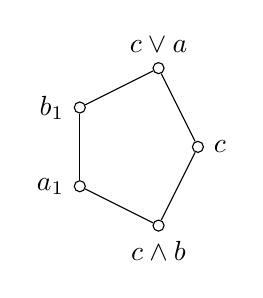
\begin{tikzpicture}
[dot/.style={circle,draw,minimum width=4pt,inner sep=1pt}]
\node[dot,label=left:$a_1$] (a) at (0,-0.5) {};
\node[dot,label=left:$b_1$] (b) at (0,0.5) {};
\node[dot,label=right:$c$] (c) at (1.5,0) {};
\node[dot,label=above:$c\vee a$] (d) at (1,1) {};
\node[dot,label=below:$c\wedge b$] (e) at (1,-1) {};
\path (d) edge (b) edge (c)
(b) edge (a) 
(e) edge (a) edge (c);
\end{tikzpicture}
\caption{}
\end{figure}
\end{proof}

\begin{theorem}[Birkhoff]
\(L\) is a nondistributive lattice iff \(M_5\), or \(N_5\) can be embedded into \(L\)
\end{theorem}

\begin{proof}
Let suppose that \(L\) is a nondistributive lattice and that \(L\) does not contain
a copy of \(N_5\) as a sublattice. Thus \(L\) is modular by Theorem \ref{thm3.5}.
Since the distributive laws do not hold in \(L\), there must be elements
\(a,b,c\) from \(L\) s.t. \((a\wedge b)\vee(a\wedge c)<a\wedge(b\vee c)\). Let
us define
\begin{align*}
d&=(a\wedge b)\vee(a\wedge c)\vee(b\wedge c)\\
e&=(a\vee b)\wedge(a\vee c)\wedge(b\vee c)\\
a_1&=(a\wedge e)\vee d\\
b_1&=(b\wedge e)\vee d\\
c_1&=(c\wedge e)\vee d
\end{align*}

Then \(d\le a_1,b_1,c_1\le e\). Now from
\begin{equation*}
a\wedge e=a\wedge(b\vee c)
\end{equation*}
and
\begin{align*}
a\wedge d&=\underline{a}\wedge(\underline{(a\wedge b)\vee(a\wedge c)}\vee(b\wedge c))\\
&=((a\wedge b)\vee(a\wedge c))\vee(a\wedge(b\wedge c))\tag*{by M}\\
&=(a\wedge b)\vee(a\wedge c)
\end{align*}
it follows that \(d<e\)

We now show that diagram in Figure \ref{fig:3.6} is a copy of \(M_5\) in \(L\). To
do this it suffices to show that 
\(a_1\wedge b_1=a_1\wedge c_1=b_1\wedge c_1=d\) 
and \(a_1\vee b_1=a_1\vee c_1=b_1\vee c_1=e\).


\begin{figure}
\centering
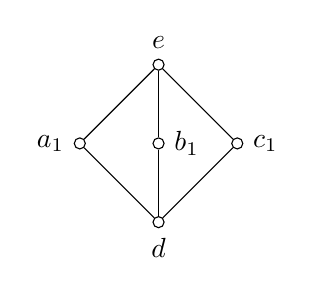
\begin{tikzpicture}
[dot/.style={circle,draw,minimum width=4pt,inner sep=1pt}]
\node[dot,label=left:$a_1$] (a) at (0,0) {};
\node[dot,label=right:$b_1$] (b) at (1,0) {};
\node[dot,label=right:$c_1$] (c) at (2,0) {};
\node[dot,label=below:$d$] (d) at (1,-1) {};
\node[dot,label=above:$e$] (e) at (1,1) {};
\path[] (e) edge (a) edge (b) edge (c)
(d) edge (a) edge (b) edge (c);
\end{tikzpicture}
\caption{}
\label{fig:3.6}
\end{figure}

\begin{align*}
a_1\wedge b_1&=((a\wedge e)\vee\underline{d})\wedge(\underline{(b\wedge e)\vee d})\\
&=((a\wedge e)\wedge((b\wedge\underline{e})\vee d))\vee d\tag*{(by M)}\\
&y\wedge z=((b\wedge e)\vee d)\wedge d=d\\
&=((a\wedge e)\wedge((b\vee d)\wedge e))\vee d\tag*{(by M)}\\
&=((a\wedge e)\wedge e\wedge(b\vee d))\vee d\\
&=((a\wedge e)\wedge(b\vee d))\vee d\\
&=(a\wedge\underline{(b\vee c)}\wedge(\underline{b}\vee(a\wedge c)))\vee d\\
&=(a\wedge(b\vee((b\vee c)\wedge(a\vee c))))\vee d\tag*{(by M)}\\
&=(\underline{a}\wedge(b\vee\underline{(a\wedge c)}))\vee d
\tag*{$a\wedge c\le b\vee c$}\\
&=(a\wedge c)\vee(b\wedge a)\vee d\tag*{(by M)}\\
&=d
\end{align*}
\end{proof}


\subsection{Complete Lattices, Equivalence Relations, and Algebraic Lattices}
\label{sec:org862677c}
\begin{definition}[]
A poset \(P\) is \textbf{complete} if for every subset \(A\) of \(P\) both \(\sup A\) and
\(\inf A\) exists in \(P\). The elements \(\sup A\) an \(\inf A\) will be
denoted by \(\bigvee A\) and \(\bigwedge A\).
\end{definition}

\begin{theorem}[]
Let \(P\) be a poset s.t. \(\bigvee A\) exists for every subset \(A\), or s.t. 
\(\bigwedge A\) exists for every subset \(A\). Then \(P\) is a complete lattice
\end{theorem}

\begin{proof}
Suppose \(\bigwedge A\) exists for every \(A\subseteq P\). Then letting \(A^u\)
be the set of upper bounds of \(A\) in \(P\), it is routine to verify that
\(\wedge A^u\) is indeed \(\vee A\).
\end{proof}

In the above theorem, the existence of \(\bigwedge\emptyset\) guarantees a
largest element in \(P\), and likewise the existence of \(\bigvee\emptyset\)
guarantees a smallest element in \(P\). (Every element is larger than
\(\emptyset\)).

\begin{definition}[]
A sublattice \(L'\) of a complete lattice \(L\) is called a \textbf{complete sublattice}
of \(L\) if for every subset \(A\) of \(L'\) the elements \(\bigvee A\) and
\(\bigwedge A\), as defined in \(L\), are actually in \(L'\)
\end{definition}

\begin{definition}[]
The \textbf{diagonal relation} \(\Delta_A\) and the \textbf{all relation} \(A^2\) is denoted by 
\(\nabla_A\). \(r_1\circ r_2\) iff there is a \(c\in A\) s.t. 
\(\la a,c\ra\in r_1\) and \(\la c,b\ra\in r_2\)
\end{definition}


\(\Eq(A)\) is the set of all equivalence relations on \(A\).

\begin{theorem}[]
The poset \(\Eq(A)\) with \(\subseteq\) as the partial ordering, is a
complete lattice.
\end{theorem}

\begin{theorem}[]
If \(\theta_1\) and \(\theta_2\) are two equivalence relations on \(A\) then
\begin{equation*}
\theta_1\vee\theta_2=\theta_1\cup(\theta_1\circ\theta_2)
\cup(\theta_1\circ\theta_2\circ\theta_1)\cup(\theta_1\circ
\theta_2\circ\theta_1\circ\theta_2)\cup\dots
\end{equation*}
or equivalently, \(\la a,b\ra\in\theta_1\vee\theta_2\) iff there is a
sequence of elements \(c_1,c_2,\dots,c_n\) from \(A\) s.t.
\begin{equation*}
\la c_i,c_{i+1}\ra\in\theta_1\quad\text{or}\quad\la c_i,c_{i+1}\ra\in\theta_2
\end{equation*}
for \(i=1,\dots,n-1\) and \(a=c,b=c_n\)
\end{theorem}

\begin{definition}[]
Let \(\theta\) be a member of \(\Eq(A)\). For \(a\in A\), the \textbf{equivalence class} (or
\textbf{coset}) \textbf{of a modulo} \(\theta\) is the set \(a/\theta=\{b\in A:\la
   b,a\ra\in\theta\}\). The set \(\{a/\theta:a\in A\}\) is denoted by
\(A/\theta\) 
\end{definition}

\begin{theorem}[]p
For \(\theta\in\Eq(A)\) and \(a,b\in A\) we have
\begin{enumerate}
\item \(A=\bigcup_{a\in A}a/\theta\)
\item \(a/\theta\neq b/\theta\) implies \(a/\theta\cap b/\theta=\emptyset\)
\end{enumerate}
\end{theorem}

\begin{definition}[]
A partition \(\pi\) of a set \(A\) is a family of nonempty pairwise disjoint subsets
of \(A\) s.t. \(A=\bigcup\pi\). The sets in \(\pi\) are called the \textbf{blocks} of \(\pi\). The
set of all partitions of \(A\) is denoted by \(\Pi(A)\)
\end{definition}

\begin{theorem}[]
\(\Pi(A)\) is a complete lattice and it's isomorphic to the lattice \(\Eq(A)\).
\end{theorem}

\begin{definition}[]
The lattice \(\Pi(A)\) is called the \textbf{lattice of partitions} of \(A\)
\end{definition}


\index{compact} \index{algebraic lattice}
\begin{definition}[]
Let \(L\) be a lattice. An element \(a\) in \(L\) is \textbf{compact} iff whenever 
\(\bigvee A\) exists and \(a\le\bigvee A\) for \(A\subseteq L\), then 
\(a\le\bigvee B\) for some finite \(B\subseteq A\). \(L\) is \textbf{compactly
generated} iff every element in \(L\) is a sup of compact elements. A lattice is
\textbf{algebraic} if it is complete and compactly generated.
\end{definition}

\subsection{Closure Operator}
\label{sec:orgf3e1735}
\begin{definition}[]
If we are given a set \(A\), a mapping \(C:\calp(A)\to\calp(A)\) is called a
closure \textbf{operator} on \(A\) if, for \(X,Y\subseteq A\) it satisfies
\begin{itemize}
\item[C1:] \(X\subseteq C(X)\)\hspace*{\fill}(extensive)
\item[C2:] \(C^2(X)=C(X)\)\hspace*{\fill}(idempotent)
\item[C3:] \(X\subseteq Y\) implies \(C(X)\subseteq C(Y)\)
\end{itemize}

A subset \(X\) of \(A\) is called a \textbf{closed subset} if \(C(X)=X\). The poset of
closed subsets of \(A\) with set inclusion is denoted by \(L_C\)
\end{definition}

\begin{theorem}[]
Let \(C\) be a closure operator on a set \(A\). Then \(L_C\) is a complete
lattice with
\begin{equation*}
\displaystyle\bigwedge_{i\in I}C(A_i)=\bigcap_{i\in I}C(A_i)
\end{equation*}
and 
\begin{equation*}
\displaystyle\bigvee_{i\in I}C(A_i)=C(\bigcup_{i\in I}A_i)
\end{equation*}
\end{theorem}


\begin{theorem}[]
Every complete lattice is isomorphic to the lattice of closed subsets of some
set \(A\) with a closure operator \(C\)
\end{theorem}

\begin{proof}
Let \(L\) be a complete lattice. For \(X\subseteq L\) define
\begin{equation*}
C(X)=\{a\in L:a\le\sup X\}
\end{equation*}
Then \(C\) is a closure operator on \(L\) and the mapping 
\(a\mapsto\{b\in L:b\le a\}\) gives the desired isomorphism
\end{proof}

\begin{definition}[]
A closure operator \(C\) on the set \(A\) is an \textbf{algebraic closure operator} if for
every \(X\subseteq A\)
\begin{itemize}
\item[C4:] \(C(X)=\bigcup\{C(Y):Y\subseteq X\text{ and } Y\text{ is finite}\}\)
\end{itemize}
\end{definition}

\begin{theorem}[]
If \(C\) is an algebraic closure operator on a set \(A\) then \(L_C\) is an
algebraic lattice, and the compact elements of \(L_C\) are precisely the closed
sets \(C(X)\), where \(X\) is a finite subset of \(A\)
\end{theorem}

\begin{proof}
First we will show that \(C(X)\) is compact if \(X\) is finite. Supppose 
\(X=\{a_1,\dots,a_k\}\) and
\begin{equation*}
C(X)\subseteq\displaystyle\bigvee_{i\in I}C(A_i)=C(\bigcup_{i\in I}A_i)
\end{equation*}
For each \(a_j\in X\) we have by (C4) a finite 
\(X_j\subseteq \bigcup_{i\in I}A_i\) with \(a_j\in C(X_j)\). Since there are
finitely many \(A_i\)'s, say \(A_{j1},\dots,A_{jn}\), s.t.
\begin{equation*}
X_j\subseteq A_{j1}\cup\cdots\cup A_{jn}
\end{equation*}
then
\begin{equation*}
a_j\in C(A_{j1}\cup\cdots\cup A_{jn})
\end{equation*}
but then
\begin{equation*}
X\subseteq \displaystyle\bigcup_{1\le j\le k}C(A_{j1}\cup\cdots\cup C_{jn})
\end{equation*}
so
\begin{equation*}
X\subseteq C(\displaystyle\bigcup_{\substack{1\le j\le k\\1\le i\le n}}A_{ji})
\end{equation*}
and hence
\begin{equation*}
C(X)\subseteq\displaystyle\bigvee_{\substack{1\le j\le k\\1\le i\le n}}C(A_{ji})
\end{equation*}
So \(C(X)\) is compact

Now suppose \(C(Y)\) is not equal to  \((C)\) for any fintie \(X\), it's not compact.
\end{proof}

\index{generating set}
\begin{definition}[]
If \(C\) is a closure operator on \(A\) and \(Y\) is closed subset of \(A\), then
we say a set \(X\) is a \textbf{generating set} for \(Y\) if \(C(X)=Y\). The set \(Y\) is 
\textbf{finitely generated} if there is a finite generating set for \(Y\). The set \(X\)
is \textbf{minimal} generating set for \(Y\) if \(X\) generates \(Y\) and no proper subset
of \(X\) generates \(Y\)
\end{definition}


\begin{corollary}[]
Let \(C\) be an algebraic closure operator on \(A\). Then the finitely generated
subsets of \(A\) are precisely the compact elements of \(L_C\)
\end{corollary}

\begin{theorem}[]
Every algebraic lattice is isomorphic to the lattice of closed subsets of
some set \(A\) with an algebraic closure operator \(C\)
\end{theorem}


\section{Index}
\label{sec:orgcf582db}
\renewcommand{\indexname}{}
\printindex
\end{document}